% -*- TeX-master: "main.tex" -*-
\begin{figure}
  \vspace{-0.2cm}
  \begin{subfigure}[h]{0.45\linewidth}
    \def\arraystretch{1.8}
    \begin{small}
      \begin{tabular}{lllcl}
        \multicolumn{5}{c}{$\lambda_u \gg \lambda_{u^*} \approx \lambda_p$} \\
        $b$ \hspace{0.05cm} & : \hspace{0.1cm} & $ \AG{S}{d^{\Trans{\Free}{1}}}, \ 
        \AG{K}{d^{\Trans{\Free}{1}}} $ &  \ @ \  & $\lambda_b$ \\
        $u$ & : & $ \AG{S}{d^{\Trans{1}{\Free}}}, \ 
                  \AG{K}{d^{\Trans{1}{\Free}}, \ x_u} $ & @ & $\lambda_u$ \\
        $u^*$ & : & $ \AG{S}{d^{\Trans{1}{\Free}}}, \ 
                    \AG{K}{d^{\Trans{1}{\Free}}, \ x_p} $ & @ & $\lambda_{u^*}$ \\
        $p$ & : & $ \AG{S}{d^{\,1}, \  x_{\Trans{u}{p}}}, \ 
                  \AG{K}{d^{\,1}} $ & @ & $\lambda_p$ \\
      \end{tabular}
    \end{small}
    % \subcaption{In Prettified Kappa}
  \end{subfigure}
  \hfill
  \begin{subfigure}[h]{0.43\linewidth}
    \begin{center}
      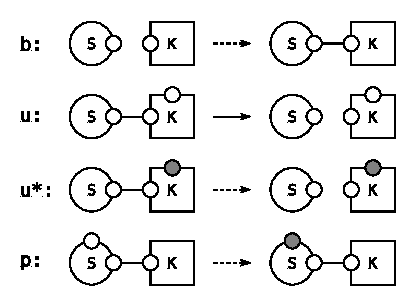
\includegraphics[scale=0.8]{kappa-diagrams/model.pdf}
    \end{center}
    % \subcaption{Graphical Representation}
  \end{subfigure}
  \caption{An Example Kappa Model. On the left, it is described using
    the \textit{edit notation} introduced in KaSim 4. Numbers in a
    rule expression correspond to local bond identifiers and $\Free$
    indicates a free site. Sites not mentioned in a rule are left
    unchanged by it. A graphical representation is provided on the
    right. Phosphorylated sites are indicated in grey. Dotted and
    solid arrows indicate \textit{slow} and \textit{fast} reactions,
    respectively.  }\label{fig:model}
\end{figure}